\section{Disk}

\subsection{Expanding on von Neumann Architecture} 

  So far, our model of the computer has been a simple von Neumann architecture which consists of a CPU and memory. However, there are many other intricacies that are extremely important in practice, and we'll expand on each one by one. 
  
  \begin{definition}[Computer Architecture]
    In our elaborated computer architecture, a computer consists of the components. 
    \begin{enumerate}
      \item A \textbf{CPU} that consists of an arithmetic logic unit (ALU), registers, and a \textbf{bus interface} that controls the input and output. 
      \item The \textbf{IO bridge} that handles communication between everything. 
      \item The \textbf{system bus} that connects the CPU to the IO bridge. 
      \item The \textbf{memory bus} that connects the memory to the IO bridge. 
      \item The \textbf{IO bus} that connects the IO devices and disk to the IO bridge. 
      \item \textbf{IO devices} like mouse, keyboard, and monitor. 
      \item The \textbf{disk controller and disk} that stores data. 
    \end{enumerate} 
    \begin{figure}[H]
      \centering 
      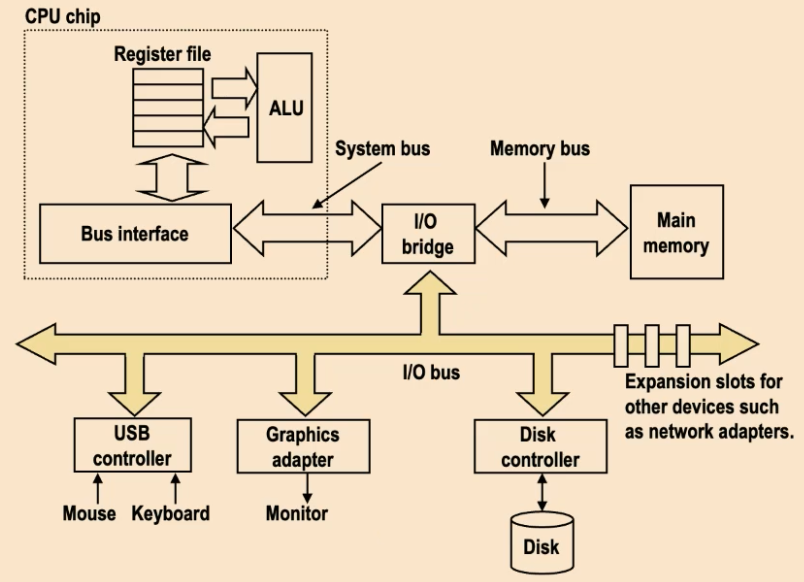
\includegraphics[scale=0.4]{img/io.png}
      \caption{Diagram of the IO bus.} 
      \label{fig:io}
    \end{figure}
  \end{definition}

  We can see from the diagram above that the CPU can directly access registers (since it's in the CPU itself) and the main memory (since it's connected to the memory bus). However, to access something like the disk, it must go through the disk controller. This gives us our first categorization of memory. 

  \begin{definition}[Primary Storage]
    \textbf{Primary storage devices} are directly accessible by the CPU and are used to store data that is currently being processed. This includes CPU registers, cache memory, and RAM. In memory, the basic storage unit is normally a \textbf{cell} (one bit per cell), which is the physical material that holds information. A \textbf{supercell} has address and data widths (number of bits), which is analogous to a lock number and the lock capacity, respectively. It is called random access since it takes approximately the same amount of time to access any cell in memory. There are two primary ways that this is implemented:  
    \begin{enumerate}
      \item \textbf{Static RAM (SRAM)} stores data in small electrical circuits (e.g. latches) and is typically the fastest type of memory. However, it is more expensive to build, consumers more power, and occupies more space, limiting the SRAM storage. 
      \item \textbf{Dynamic RAM (DRAM)} stores data using electrical components (e.g. capacitors) that hold an electrical charge. It is called \textit{dynamic} because a DRAM system must frequently refresh the charge of its capacitors to maintain a stored value. It also requires error correction which introduces redundancy. 
    \end{enumerate}

    \begin{table}[H]
      \centering
      \begin{tabular}{|l|l|l|l|}
      \hline
      \textbf{Device} & \textbf{Capacity} & \textbf{Approx. latency} & \textbf{RAM type} \\ \hline
      Register & 4 - 8 bytes & < 1 ns & SRAM \\ \hline
      CPU cache & 1 - 32 megabytes & 5 ns & SRAM \\ \hline
      Main memory & 4 - 64 gigabytes & 100 ns & DRAM \\ \hline
      \end{tabular}
      \caption{Memory hierarchy characteristics}
      \label{tab:memory_hierarchy}
    \end{table}
  \end{definition}

  \begin{definition}[Secondary Storage]
    \textbf{Secondary storage devices} are not directly accessible by the CPU and are used to store data that is not currently being processed. This includes hard drives, SSDs, and magnetic tapes. There are two primary ways: 
    \begin{enumerate}
      \item \textbf{Spinning disks} store data on a magnetic surface that spins at high speeds.
      \item \textbf{Solid state drives (SSDs)} store data on flash memory chips.
    \end{enumerate}
  \end{definition}

  There are three key components of memory that we should think about: 
  \begin{enumerate}
    \item The \textbf{capacity}, i.e. amount of data, it can store (how large the water tank is). 
    \item The \textbf{latency}, i.e. amount of time it takes for a device to respond with data after it has been instructed to perform a data retrieval operation (how fast the data flows). 
    \item The \textbf{transfer rate} or \textbf{thoroughput}, i.e. amount of data that can be moved between the device and main memory (how wide the pipe is). Naively, with one channel and sequential transfer the transfer rate is one over the latency. 
  \end{enumerate}

  We must provide a good balance of these three qualities, and also note that there are some physical limitations (i.e. latency cannot be faster than speed of light), and this is more effectively done through a hierarchical memory system.

  \begin{figure}[H]
    \centering 
    \begin{tabular}{|l|c|c|}
      \hline
      \textbf{Storage Type} & \textbf{Access Time} & \textbf{Category} \\
      \hline
      Registers & 1 cycle & Primary Storage \\
      \hline
      Caches & $\sim$10 cycles & Primary Storage \\
      \hline
      Main Memory & $\sim$100 cycles & Primary Storage \\
      \hline
      Flash Disk & $\sim$1 M cycles & Secondary Storage \\
      \hline
      Traditional Disk & $\sim$10 M cycles & Secondary Storage \\
      \hline
      Remote Secondary Storage & Depends on Latency & Secondary Storage \\
      (e.g., Internet) & & \\
      \hline
    \end{tabular}
    \caption{Memory hierarchy.} 
    \label{fig:memory_hierarchy}
  \end{figure}

  For example when we want to read from the disk, the CPU must request to the bus interface, which travels through the bus interface, I/O bridge, I/O bus, disk controller, and to the disk itself. Then the data goes back through the disk controller, I/O bus, I/O bridge, through the memory bus, and resides in the main memory. Note that disks are block addressed, so it will transfer the entire block of data into the memory. It must specify a \textbf{destination memory address (DMA)}. When the DMA completes, the disk controller notifies the CPU with an \textit{interrupt} (i.e. asserts a special interrupt pin on the CPU), letting it know that the operation has finished. This signal goes through the disk controller to the IO bridge to the CPU. From now on, the CPU knows that there is memory that it can access to run an application loaded in memory. 

\subsection{Disk} 

  \begin{definition}[Hard Disk Drives]
    Back then, there were \textbf{hard disk drives (HDDs)} that literally had a spinning wheel and a needle head that read the data. 
    \begin{figure}[H]
      \centering 
      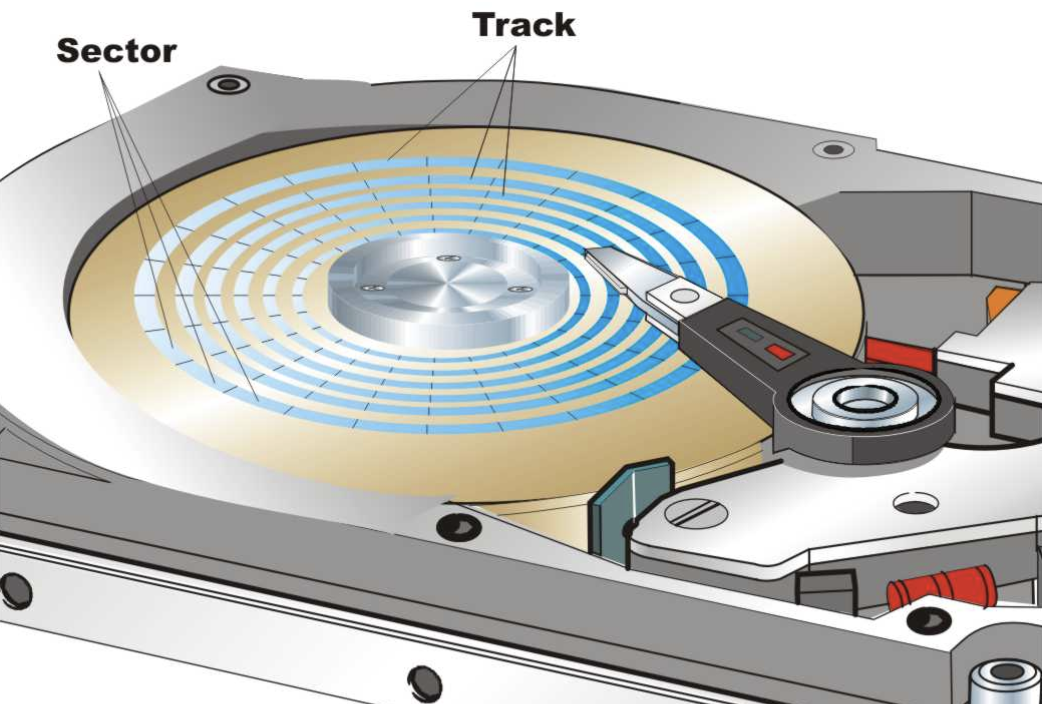
\includegraphics[scale=0.4]{img/hdd.png}
      \caption{Visual diagram of hard disk drive with its sectors. } 
      \label{fig:hdd}
    \end{figure}
    \begin{enumerate}
      \item HDDs are not random access since the data must be sequentially read. This was disadvantageous since the spinning wheel had to spin to the correct location, which took time. The needle also had to move to the correct location, which also took time and therefore read and write speeds were dominated by the time it took to move the needle.
      \item The smallest unit of data that can be read is a complete disk sector (not a single byte like RAM). 
    \end{enumerate}
  \end{definition}

  \begin{definition}[Solid State Drives]
    Now, we have \textbf{solid state drives (SSDs)} that store data on flash memory chips. This is advantageous since there are no moving parts, so the latency is much lower and the latency is not dominated by the time it takes to move the needle. 
    \begin{enumerate}
      \item SSDs are random access. 
      \item The smallest unit of data is a \textbf{page}, which is usually 4KB and maybe for high scale computers 2-4 MB (but on ``Big Data'' applications big but computers, it can be up to 1GB). 
      \item A collection of pages, usually 128 pages, is called a \textbf{block}, making is 512KB. 
    \end{enumerate}
  \end{definition}

  While virtually all RAM and primary storage devices are \textbf{byte addressable} (i.e. you can access any byte in memory), secondary storage devices are \textbf{block addressable} (i.e. you can only access a block of memory at a time). Therefore, to access a single byte in secondary storage, you must first load the entire block into memory, calculate which byte from that block you want, and then access it. Therefore, you need both the block number $x$ and the offset $o$ to access a byte in secondary storage, which is why it is even slower than accessing RAM. 

  \begin{figure}[H]
    \centering 
    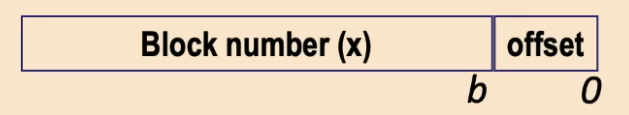
\includegraphics[scale=0.4]{img/block_offset.png}
    \caption{Block offset.} 
    \label{fig:block_offset}
  \end{figure}

  Therefore, you can think of raw data in units of blocks of size $2^b$ for some $b$ bits. 
  \begin{enumerate}
    \item Take the low order $b$ bits of a byte address as an integer, which is the offset of the addressed byte in the block. 
    \item THe rest of the bits are the block number $x$, which is an unsigned long. 
    \item You request the block number $x$, receive the block contents, and then extract the requested byte at offset in $x$ i.e. calculate \texttt{block[x][offset]}. 
  \end{enumerate}

